\documentclass[11pt,a4paper]{article}
\usepackage{url}
\usepackage{graphicx}

 \renewcommand{\familydefault}{\sfdefault}

\begin{document}
\title{Runner - A Cyberpunk Roguelike}
\author{M. Fink}

\maketitle

% \begin{abstract}
% A primer for my upcoming cy
% \end{abstract}

\section{Introduction}
This document is a short primer, an exploration of ideas towards the game I want to create.
Design is a very fleeting, fluid process, none of this is written in stone. But pouring
thoughts into text, helps to steer a creative vision.
One of the biggest dangers when doing creative work is overambition, and in Game Design
feature creep. That is why I am formulating three design pillars: to prevent a loss of
focus by adding to many things that just leave a muddy chaotic mess. With everything added
to the game, the question should be, does it strengthen one of these pillars.

\section{Setting and Atmosphere}
\textit{The setting is very much a blank slate, but I'll try to give some kind of seed.}
I definitely know the tone and atmosphere I want to set. The setting should be dark,
rainy and reference contemporary problems, extrapolated in a slightly exaggerated way.
The tone should be serious at times, but not fully grimdark at all times. A lot of
cynical humor and caricative exagerrating should contrast the bleakness of struggling
future mankind. There is one work of fiction that exactly nails this tone:
\textit{Neal Stephenson: Snow Crash}

The story focus should lie more on the way humans get lost in a progressing technological
world, the alienation of individual humans, the eternal struggle between the rich and
poor, and fear of the future. This is not about the marvels of technology that might come.
We are some dozen years into the future and the dreams of interplanetary space travel
and superhuman AI seem closer than ever, but just out of reach.

The unstoppable progress of the 21st century starts to stutter due to environmental
destruction, increasingly chaotic economy crises and a general disregard for human
needs. Will the deciding technological jump occur, that solves these problems once and
for all? Will there be a Watt, Edison or Musk to trigger the necessary jump in evolution?
This might well be the decade, that once and for all decides the fall, or rise of the
human race.

\section{Game Design Pillars}
\begin{itemize}
    \item \textbf{Multiple Level solution approaches:
        Fight, stealth, talk should all be viable, equally effective options}
        This is not a game about min-maxing stats or grinding XP. Each level should be a
        playground, a sandbox puzzle that lets you choose how to solve it - keeping the spirit
        of \textit{Deus Ex}, or Warren Specter's \textit{One block sim}.

    \item \textbf{Complex, Interconnected and deeply simulated levels:
        via Lock-Key-puzzles, hackable Computer Networks, lighting and physics systems.}
        To offer an interesting Sandbox with multiple approaches, there should be lots of system
        interacting in consistent and believable ways. The design explicitly puts few small, but
        complex and deeply interconnected levels above a huge number of dungeon floors and enemy
        types.

    \item \textbf{Lively NPCs:
        Talkative and interactive AI with backstories, emotional states and relationships.}
        This will support the humanizing part of the theme. NPC's should be more than just cannon
        fodder. You should be encouraged to go the stealthy and non-violent routes, not because You
        get more XP or loot, but because NPC's have a 'life' and deserve empathy.
\end{itemize}

\section{Vision and Inspirations}
Common knowledge has it that every creative endeavour is mostly clever copying and remixing, so I'll
just honestly state my sources and Inspirations. I want to keep the list short, although I know there
is way more Cyberpunk material out there. But these works contain the aspects I especially want to
focus on:\\ \

\textbf{Movies and Books}

\begin{itemize}
    \item \textbf{Mr. Robot}: A bleak version of mankind, where everyone forgot how to connect to people,
            everyone is working for his goals. The more power, the more egocentric. And there's
            always a darker and more powerful force pulling the strings.
    \item \textbf{Ghost in the Shell}: A softer, more melancholic look on a mankind slowly forgetting it's
            humanity. If you take your time meditate and listen, there's still some places of silent
            beauty between the towering slums.
    \item \textbf{Snow Crash}: Some aspects of the world always evolve beyond anything that parody could come
            up with. The church operating on corporate principles? The Mafia becoming a
            well-established and respected brand? Pizza deliverators are treated as outlaws?
            It all sounds very stupid, but hasn't the last decade taught us, that economy and politics
            can bring nasty surprises that overshadow everything a cynical comedian could dream of?
\end{itemize}

\textbf{Games}

\begin{itemize}
    \item \textbf{Monaco}: My initial pitch would have been: I want to do Monaco, but with a bit of a more serious
                background, more Cyberpunky, a bit less chaotic, a bit more deliberate. I really adore how all
                the systems in this game interact and let you play with, so this idea still stands deep in the
                core of my vision.
    \item \textbf{Invisible Inc}: Has shown, that good stealth gameplay doesn't necessarily have to be realtime
                and can work well with procedural generation. The game design is tightly focused on a small
                of tools and interactions. And the
    \item \textbf{Deus Ex}: What do I need to say here? Dark rainy world, poor lonely people, stealth,
                social engineering, high tech waponry -- They have it all. Still, Deus Ex always lacked a proper representation of
                what 'hacking' actually means. It's not about solving samey logic puzzles. Hacking is about creativity.
                About playfully misusing the systems and tools that you are given.
\end{itemize}

\section{Gameplay Loop}

\begin{figure}
    \center
    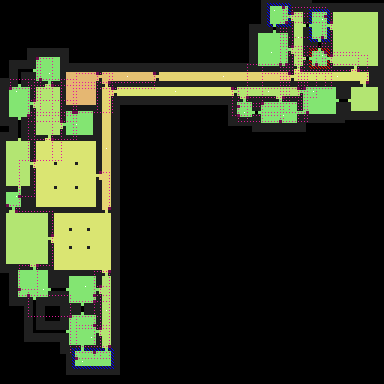
\includegraphics[width=0.47\textwidth]{level1.png}
    \hfill
    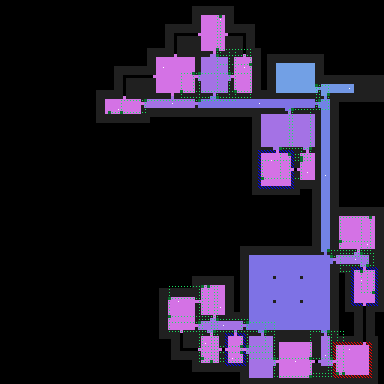
\includegraphics[width=0.47\textwidth]{level2.png}

    \vspace{0.5cm}

    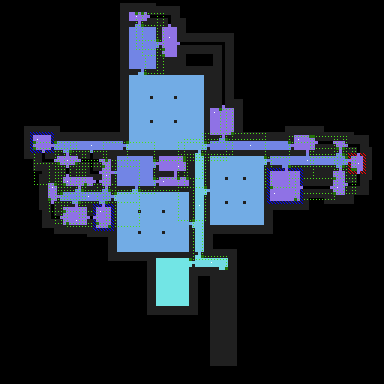
\includegraphics[width=0.47\textwidth]{level4.png}
    \hfill
    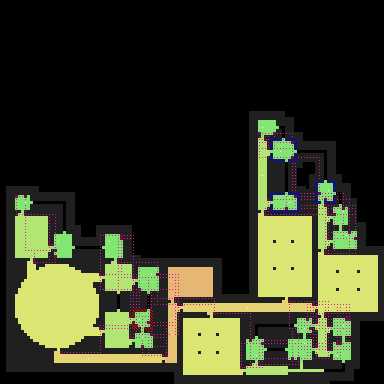
\includegraphics[width=0.47\textwidth]{level3.png}

    \caption{Some results of the level generator, with procedural color palettes and cross-, ring- or corner-shaped
            level footprints.}
\end{figure}

For the beginning, the main gameplay loop will be the typical heist trope. You start at the periphery of the level.
You get to the vault, with whatever means necessary. That first means careful exploration of the outer parts of the
level, and and the preparing to penetrate into the inner high security zones.
The tools you can find in the level are physical, like weapon prototypes, industrial tools or machines. But they can
also be humans, that may be convinced or bribed to give you keys or information. Or you find your tools in the
\textbf{GRID}, the virtual layer that meshes together all smart things in the facility. A parallel space to explore
and trigger repercussions into the meat world.
However, the facility is aware of you. The more mess you make, the more lifes you take, the harder it will resist.
Alarm levels will increase for every 'noisy' action you take, and security presence will become impregnable if you're
not careful. Maybe at one point during your run the priorities change, and your new goal will be to
\textit{just get out alive}.\\  \

\textit{For the far future:} Maybe the level generator also lends itself to create a hub level, the \textit{Arcology}, to add
some metagame in between individual runs. But this will be only considered when one facility run is playable from
insertion to extraction.

% \section{Game World}
%
% \textit{preliminary}
%
%



\end{document}
